\chapter{実験}
\label{experiment}
%仮説を検証するためにやったことを再現可能な様に書く
%結果も書く

本章では提案手法の実験について述べる。

\section{概要}
\label{sub:実験概要}
本研究の仮説をもとに、システムの実装をおこなった。
\begin{figure}[h]
  \begin{center}
      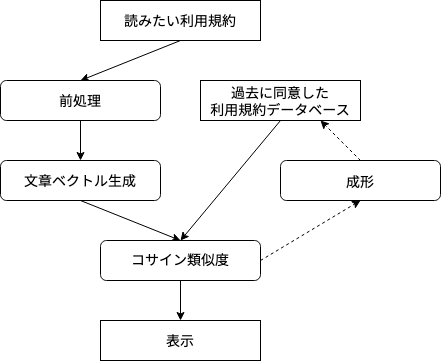
\includegraphics[width=10cm]{img/system.drawio.png}
      \caption{類似条文検出の実装イメージ}
      \label{img:類似条文検出の実装イメージ}
  \end{center}
\end{figure}

各節にて、図\ref{img:類似条文検出の実装イメージ}に基づいた実装の詳細について説明をする。利用規約を表示した際に出てくる各条項を「読みたい利用規約」として分解を行う。それぞれの条項に対して、図\ref{img:類似条文検出の実装イメージ}のシステムを通し、表示を行う。なお、本章では利用規約の項や号についてを条項と表現する。

\section{前処理}
\label{sec:前処理}
まず、読みたい利用規約について前処理を行う。これは、条項が自然言語処理を行うために適さない文章である場合があるためである。具体的には、正規表現を利用し、以下のような処理を行なった。

\begin{itemize}
  \item 空白の除去
  \item URLの除去
  \item かっこ(「」、()など)の除去
  \item 「ユーザー」「ユーザ」「利用者」などの表現の統一
  \item 社名の置き換え
\end{itemize}

以上は処理の例である。このような処理を通して、類似度の精度の向上を行う。

\section{文ベクトル生成}
類似度を求めるために、文ベクトルの生成を行う。文章ベクトルの生成には、質問モデルなどで精度の高かったSentence-BERTを利用する。また、日本語の事前学習モデルについては、芝山ら\cite{weko_212207_1}の研究において精度が高かった、東北大版のBERT\footnote{https://github.com/cl-tohoku/bert-japanese}をもとに生成されたSentence BERTモデル\footnote{https://huggingface.co/sonoisa/sentence-bert-base-ja-mean-tokens-v2}を利用して生成を行う。

\section{コサイン類似度}
生成した文ベクトルは、以下の式でコサイン類似度を求めることにより、与えられた文同士の意味の近さを数値化することができる。
$$sim = \frac{x\cdot y}{|\bar{x}||\bar{y}|}$$
本研究では、この数値をScoreとして最終的に表示を行う。また、この数値を一定の閾値において表示の目立たせる切り替えを行う必要がある。閾値に関しては、実際に利用規約の表示を行い比較を行ったところ、$score=0.89$を閾値としている。この値は、モデルの差異などによっても異なっているため、さらに調整が必要になる可能性がある。

\section{成形}
\label{sec:成形}
類似度の表示を行なった後に、今後読む利用規約のために、過去に同意した利用規約データベースに追記を行う。(なお、この処理は、利用規約に「同意する」ボタンをクリックした場合について行い、「同意しない」ボタンをクリックした場合は追記を行わない。)\ref{sec:前処理}節での処理などが十分に行われているのかを確認し、データベースに追記する問題がないことの確認を行う。おおむねは\ref{sec:前処理}節での処理で十分であることが多いが、様々な利用規約を調査したところ、これらの処理では不十分な場合があり、これ以外にも前処理を手作業で行なった部分がある。以下にその例を示す。

\begin{itembox}[l]{モイ株式会社 サービス利用規約 第3条第1項}
  モイは,本サービス運営上の合理的必要性があるとモイが判断した場合,本利用規約を変更できるものとします。
\end{itembox}  

モイ株式会社のサービス利用規約においては、全文にわたってモイ株式会社について「モイ」もしくは「当社」と表現している。「モイ」のままであると類似度を求めるにあたって不都合なため、「当社」と置き換える処理を行う。これらに関して、固有表現抽出を使用して社名を認識することができるのではないかと検討を行ったが、以下のような利用規約では適用できないことが判明した。

\begin{itembox}[l]{株式会社Z会ソリューションズ 利用規約}
  ユーザがクレジットカード決済、コンビニ決済を選択した場合、当社は請求業務をGMOペイメントゲートウェイ株式会社に委託できるものとします。
\end{itembox}

このような利用規約の場合、「GMOペイメントゲートウェイ株式会社」のような表現がある場合、これについても会社名と認識してしまう場合がある。このとき、一般的な利用規約の場合は「当社は請求業務を代行業社に依頼することができる」といった表現になるため、これらについての置き換えは現状困難であると考えられる。よって、これらについて手作業を入れて確認を要する。

\section{過去に同意した利用規約データベース}
\ref{sec:成形}節において問題なく成形された条項に関して、その後に読む利用規約と比較するためにデータベースへの登録を行なう。データベースへは以下の情報を登録する。

\begin{table}[h]
  \centering
  \caption{過去に同意した利用規約データベースの内容}
  \begin{tabular}{cc}
  \hline
  形式                      & 項目                    \\ \hline \hline
  数値                      & 条項ID                     \\ \hline
  数値                      & 条項の形式\tablefootnote{条項であるか、第n条などの見出しであるかを区別する。見出しは文ベクトルの生成を行わず、類似度の比較も行わない。}                     \\ \hline
  文字                      & 条項                        \\ \hline
  ベクトル                    & 条項の文ベクトル                  \\ \hline
  \end{tabular}
\end{table}
データベースに文ベクトルを保存しておくことにより、効率的に類似度の計算を行うことができる。

なお、「同意しない」を選択した利用規約の条項に関してはデータベースへの登録は行わない。

%図\ref{img:類似条文検出の実装イメージ}に示したように、まず、読みたい利用規約について、前処理を行う。ここでは、URLの置き換え、かっこなどの記号の除去、「利用者」「会員」などを「ユーザー」に表現を揃えるなどの処理を行う。また、条文と条文でない部分(「第○条」、「以上」のような表現など)を除去するための情報がここで与えられる。本研究では、条文でない部分に関しての情報はあらかじめ手作業で与えることとした。その後、文章ベクトルを生成する。本研究では、東北大乾研の大規模日本語モデルを利用した。そして、生成された文章ベクトルと過去に同意した利用規約データベースに保存されている文ベクトルとコサイン類似度の計算を行い、表示する。表示したのち、利用者が同意をした場合は、文章の成形、保存された文章に前処理で取り除けなかった余分な情報などが含まれないかを確認し、必要であれば編集と文章ベクトルの再生成を行い、過去に同意した利用規約データベースに保存する。その情報が増えることにより、検出される条文が増える。同意しなかった場合は保存をしない。

\section{利用規約警告検出}
利用規約警告検出についても同様の処理を行う。なお、閾値を超えた場合に文を目立たせる処理を行うため、上記までと逆の判定をおこなっている。

\section{表示方法}
表示方法については、利用規約の類似条文検出に加えて、判断の材料にするために、類似度の高い順に3つの条文とその条文をもつサービス名、コサイン類似度を表示した。3つに設定した根拠としては、他サービスの条文と比較するときに複数サービスの条文と比較することで、より類似度を利用者が比較しやすいと考えたからである。

また、利用規約を目立たせる表示として、一定の閾値のコサイン類似度を超えた背景をオレンジ色とすることにした。

利用規約警告検出は、オレンジ色と区別をできるように、水色とした。また、この区別は利用者が能動的に指定をおこなっているため、類似条文検出よりも優先して表示をおこなっている。

\begin{figure}[h]
  \begin{center}
      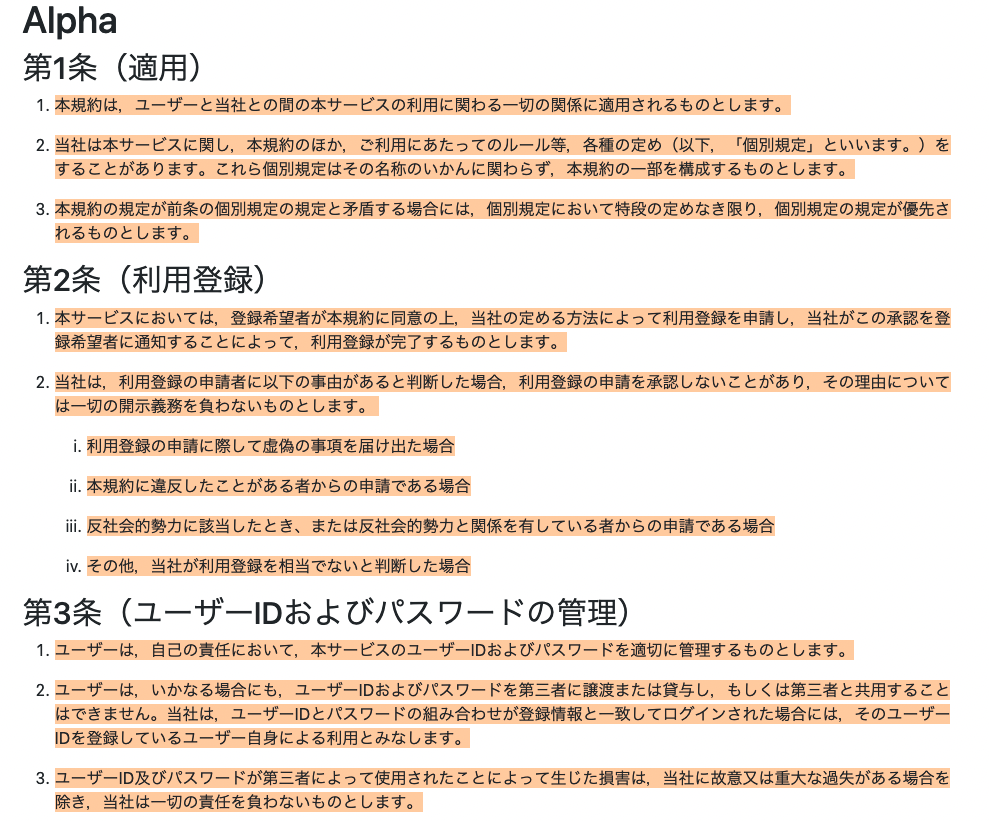
\includegraphics[width=16cm]{img/alpha.png}
      \caption{Alpha社の利用規約/どの利用規約も既読ではない}
      \label{img:Alpha社の利用規約/どの利用規約も既読ではない}
  \end{center}
\end{figure}
\begin{figure}[h]
  \begin{center}
      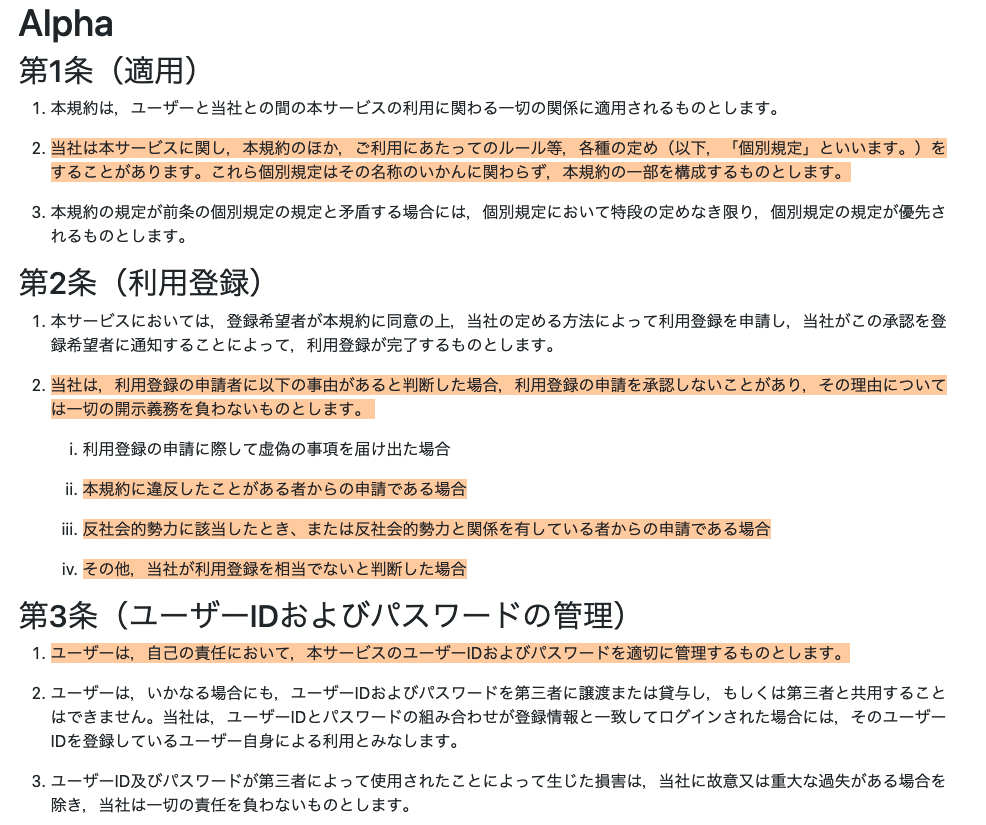
\includegraphics[width=16cm]{img/alpha_b.png}
      \caption{Alpha社の利用規約/Beta社が既読}
      \label{img:Alpha社の利用規約/Beta社が既読}
  \end{center}
\end{figure}
\begin{figure}[h]
  \begin{center}
      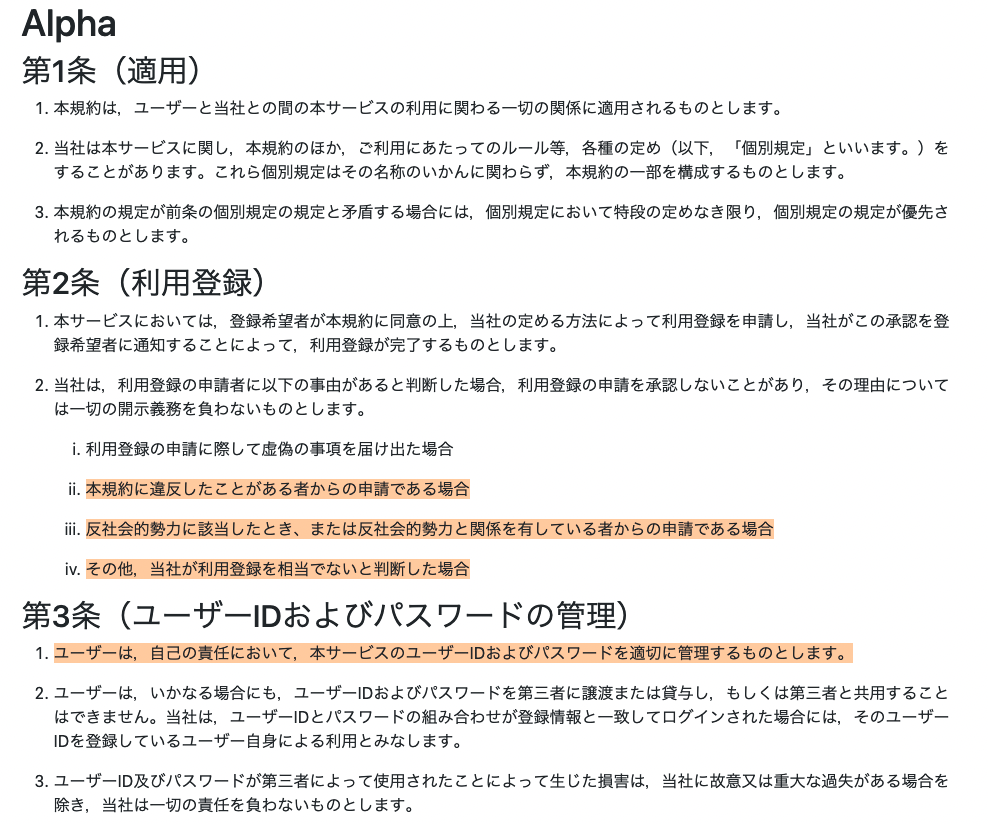
\includegraphics[width=16cm]{img/alpha_bg.png}
      \caption{Alpha社の利用規約/Beta社、Gamma社が既読}
      \label{img:Alpha社の利用規約/Beta社、Gamma社が既読}
  \end{center}
\end{figure}
\begin{figure}[h]
  \begin{center}
      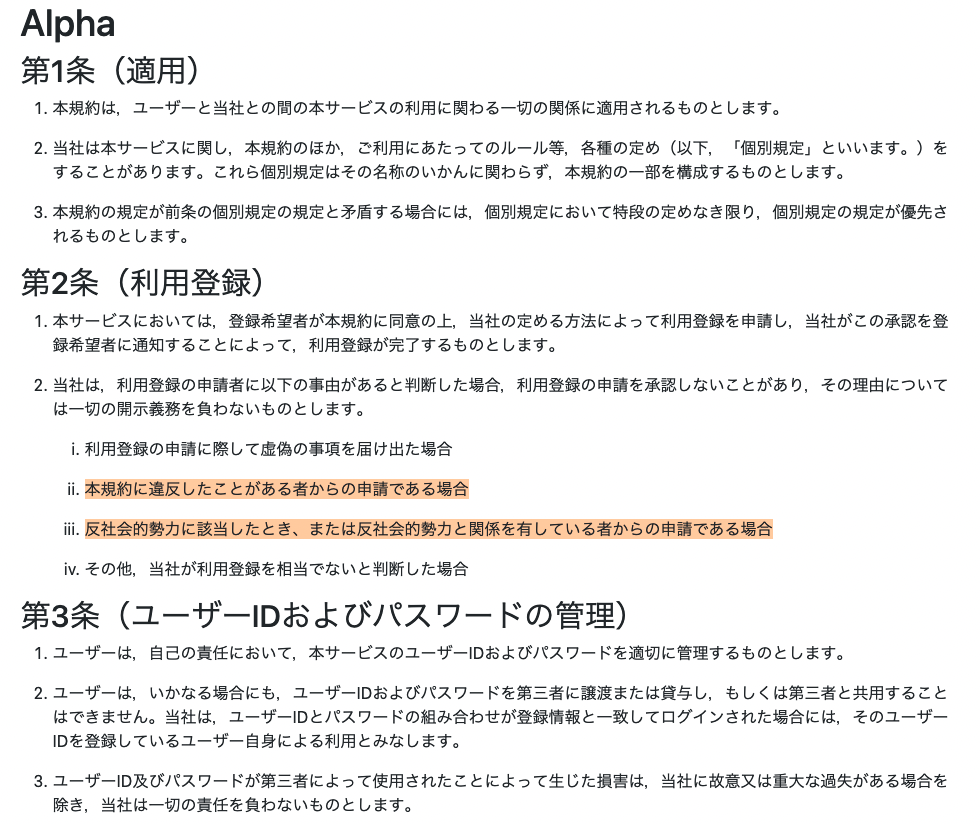
\includegraphics[width=16cm]{img/alpha_bgd.png}
      \caption{Alpha社の利用規約/Beta社、Gamma社、Delta社が既読}
      \label{img:Alpha社の利用規約/Beta社、Gamma社、Delta社が既読}
  \end{center}
\end{figure}

利用規約3つのスコア表示と利用規約警告表示の図を追加する。

%\section{実行環境}
%\begin{center}
%  \begin{tabular}{ll} \hline
%    項目 & 仕様 \\ \hline \hline
%    環境 & Azure Web App Service\\
%    インスタンス & B1 \\
%    コア数 & 1 \\
%    RAM & 1.75GB \\ \hline
%  \end{tabular}
% \end{center}

%%% Local Variables:
%%% mode: japanese-latex
%%% TeX-master: "../bthesis"
%%% End:
